\documentclass[conference]{IEEEtran}
\IEEEoverridecommandlockouts
% The preceding line is only needed to identify funding in the first footnote. If that is unneeded, please comment it out.
\usepackage{cite}
\usepackage{amsmath,amssymb,amsfonts}
\usepackage{algorithmic}
\usepackage{graphicx}
\usepackage{textcomp}
\usepackage{xcolor}
\usepackage{hyperref}
\hypersetup{
    colorlinks=true,
    linkcolor=blue,
    filecolor=blue,      
    urlcolor=blue,
    pdftitle={Overleaf Example},
    pdfpagemode=FullScreen,
    }

\usepackage{listings}
\usepackage{xcolor}

\lstdefinelanguage{Rust}{
  morekeywords={
    as, break, const, continue, crate, else, enum, extern, false, fn, for,
    if, impl, in, let, loop, match, mod, move, mut, pub, ref, return, self,
    Self, static, struct, super, trait, true, type, unsafe, use, where, while,
    async, await, dyn
  },
  sensitive=true,
  morecomment=[l]{//},
  morecomment=[s]{/*}{*/},
  morestring=[b]{"}
}

\lstdefinestyle{ruststyle}{
  language=Rust,
  backgroundcolor=\color{gray!10},
  commentstyle=\color{green!60!black},
  keywordstyle=\color{blue},
  numberstyle=\tiny\color{gray},
  stringstyle=\color{orange},
  basicstyle=\ttfamily\footnotesize,
  breaklines=true,
  numbers=left,
  numbersep=5pt,
  showstringspaces=false,
  tabsize=2,
  captionpos=b
}

\lstset{style=ruststyle} 

\def\BibTeX{{\rm B\kern-.05em{\sc i\kern-.025em b}\kern-.08em
    T\kern-.1667em\lower.7ex\hbox{E}\kern-.125emX}}
\begin{document}

\title{
Deep Learning Implementation With Rust \\
{
\footnotesize \href{https://github.com/tung-ngt/ml-rs}{Implementation Link}
}
}

\author{
\IEEEauthorblockN{Nguyen Thanh Tung}
\IEEEauthorblockA{2440047}
}

\maketitle

\begin{abstract}
With the accelerating development of Deep Learning, particularly in 
Computer Vision and Natural Language Processing with LLM.
We have became dependent on Deep Learning frameworks like PyTorch\cite{pytorch} from MetaAI or TensorFlow from Google Brain.
Both of which are high-level frameworks providing abstractions upon Deep Learning primitives.
The two frameworks' backends are implemented using C/C++ and provide python bindings.
The high level of abstraction of these frameworks is crucial for fast and rapid prototyping.
However, the abstractions come at the cost of explicitness.
For instance, the backward propagation operation is often elided and left handle by autograd.
Although both PyTorch and TensorFlow\cite{tf} do offer ways for user to self-implement autograd functions; these methods are not fully supported as the builtin autograd functions.
Moreover, the culmination of backends implemented using C/C++ (which are memory unsafe languages) and python (which is dynamically typed) can make the runtime behaviors hard to predict.
Therefore, in this paper, we introduce a new Deep Learning framework fully implemented from scratch in Rust (a memory safe, robustly typed, high-performing language) providing explicit and modular APis for Deep Learning processes.

\end{abstract}

\begin{IEEEkeywords}
Deep Learning, Framework Implementation, Explicit and Modular API, Rust, Memory Safe.
\end{IEEEkeywords}

\section{Introduction}
Frameworks such as PyTorch\cite{pytorch}, TensorFlow\cite{tf} have been an inseparable part of developing, training, and inferring of Deep Learning models. They have become increasingly important because of the accelerating research and development of new foundation models.

Both of these frameworks provide user with high-level APIs for Deep Learning primitives like modules, operation, optimizer, loss function. 
Although these high-level APIs let researchers and developers quickly experiments with different model architectures and rapidly produce prototypes; however, these abstractions can pose as obfuscations of the mathematics and inner-working of models.
For instance, both PyTorch and TensorFlow employ different methods of automatic differentiation which are very beneficial to quickly developing models but they can be an obstacle when you want to explicitly and specifically control the flows of gradient.

Moreover, the frameworks are implemented in C/C++ which are memory unsafe languages.
Without proper handle of memory, we can observed undefined behavior at the model runtime and worse bad actor can use it as attack factors.
Although these frameworks are robustly tested and maintained by a skilled team of researchers and developers; we can not guarantee that there will never be memory-related bugs.
In additions, these frameworks provide the fronted bindings in Python which provide a user-friendly API for rapid development; however, the dynamically typed nature of this language make the it cannot be checked at compile time and can produce unwanted behavior at runtime.

In this paper, we give implementation details to a new Deep Learning framework built from scratch with no dependency in a single memory safe and robustly type language Rust. The framework provides a intermediate level API to Deep Learning primitives. The framework makes no over abstraction and exposes all the mathematical inner-working which is advantageous for fully controlling the model and research.

The paper is structured with the following sections:
\begin{itemize}
    \item Related Works.
    \item Tensor and Linear Algebra Implementation.
    \item Deep Learning Primitives.
    \item Layers Implementation.
    \item Losses Implementation.
    \item Optimizers Implementation.
    \item Dynamic Model Architecture Loading.
    \item Random Generator Implementation.
    \item Data Loading and Metrics Implementation.
    \item Experiments and Results.
    \item Challenges and Future Works.
\end{itemize}


\section{Related Works}

\subsection{PyTorch}
In recent years, PyTorch has become a leading platform for developing state-of-the-art machine learning models. PyTorch is an open-source deep learning framework developed by Meta AI that provides a flexible Python interface for building and training neural networks. Moreover, PyTorch has high performance due to its optimized implementation in C/C++. PyTorch is very flexible due to its dynamic computation graph. PyTorch allows users to define and modify models on the fly without having to explicitly specify the derivatives, making prototyping faster. The core of the PyTorch architecture is the dynamic computation graph. Tensors in PyTorch can record operations done on them dynamically to build a computation graph on the fly. The computation graph is used automatic differentiation in the backward pass. 

\subsection{TensorFlow}
TensorFlow is an open-source machine learning framework developed by Google that enables the development and deployment of scalable and high-performance models across a wide range of platforms, including desktops, servers, mobile devices, and edge systems. It offers a high level API similar to PyTorch but with functional paradigm. TensorFlow uses static computation graphs, which can be optimized for speed and efficiency. The computation graph is compiled once when we build the model which allow for better optimization.

In contrast to the graph building paradigm of the PyTorch and TensorFlow for automatic differentiation, our implementation use a semi-automatic differentiation. We provide a range of building block layer which implement both forward and backward. The user is in full control and can explicitly manage the flow of gradients when doing backpropagation.

\section{Tensor and Linear Algebra Implementation}
\subsection{Tensor Definition}
In linear algebra, we can organize numbers (of a set, usually \(R\) in Deep Learning) in different structures.
For example, we can organize numbers (scalers) in one direction (dimension) row or column to form a vector.
We can also stack rows on top of each other or columns next together for two dimension which create a matrix.
Organizing number in these structures provides a concise mathematical framework for formulating and operating on a large number of numbers easily.

A tensor extends this concept into n dimensions. The shape of a tensor is a tuple of n positive integer number, each number represent the number of addressable index in that dimension. 
A number in a n dimensions tensor can be addressed with n index numbers along n directions.

\begin{equation}
shape(T) = (s_0,s_1,...,s_{n -1}),  s_i \in N^*\label{tensor-def}
\end{equation}

\begin{equation}
T[idx_0,idx_1,...,idx_{n-1}] = a, idx_i \in [0,s_i-1],a\in R \label{tensor-def}
\end{equation}

\subsection{Tensor Implementation}
\subsubsection{Data Layout}
Although a tensor has n dimensions, to store it on a computer, we flattened it to one dimension: a single array.
The total number of elements in the flatten array will be the product over the shape of the tensor.
We store the elements in with respect to the dimension order. The last dimension is the fastest changing dimension and the first dimension is the slowest changing dimensions.

\subsubsection{Strides and Indexing}
To index into the n dimensions tensor, we need to use the its n strides. A stride of a tensor dimension is the number of elements in the flattened array, we must move over to go to the next index in that dimension.

\begin{equation}
\begin{split}
strides(T) &= (strd_0, ..., strd_{n-1}) \\
strd_i &= \prod_{k=i+1}^{n-1}s_k \\ 
strd_{n-1} &= 1
\end{split}\label{strides}
\end{equation}
\begin{equation}
\begin{split}
idx_{flattened} &= \sum_{i=0}^{n-1} strd_i\times idx_i\\
T[idx_0,...,idx_{n-1}] &= T_{flattened}[idx_{flattened}]
\end{split}\label{flatten-idx}
\end{equation}

\subsubsection{Tensor Metadata, Subtensor and Tensor Immutability}
In Deep Learning, many tensor is reused and/or taken sub-sections such as the data and label tensors.
Therefore, it is beneficial to save memory by letting many tensor and subtensor to point to the same flattened data array with only different metadata.

The metadata of a tensor includes: shape, strides, pointer to flattened data array, offset to the first element inside the data array.

With this scheme when we want to copy a tensor, we only need to copy the metadata instead of the whole data array (which is computationally expensive). When we want to use a subsection of a tensor, we can just change the shape and offset while keeping the strides and the pointer to the data array.

Moreover, as many tensors can be point to the same data array, we must ensure that the data is not mutable to ensure correctness between tensors. Every mutation operation must result in a new tensor with a new data array instead of modifying the old one.
\subsection{Linear Algebra Implementation}
In order to effectively use tensors for Deep Learning purposes, we have implemented some basic operation:
\subsubsection{Matrix multiplication}
\begin{equation}
\begin{split}
&A, B \text{  are 2d tensors}\\
&C = AB\\    
&C[i,j] = \sum_k A[i,k][k,j]
\end{split}\label{matmul}
\end{equation}

\subsubsection{Tensor addition}
\begin{equation}
\begin{split}
C &= A + B\\    
C[idx_0,...,idx_{n-1}] &= A[idx_0,..., idx_{n-1}] \\ &+B[idx_0,..., idx_{n-1}]
\end{split}\label{add}
\end{equation}

\subsubsection{Scaling}
\begin{equation}
\begin{split}
C &= \alpha A \\    
C[idx_0,...,idx_{n-1}] &= \alpha A[idx_0,..., idx_{n-1}]
\end{split}\label{scale}
\end{equation}

\subsubsection{Tensor Transpose}
\begin{equation}
\begin{split}    
&idx_i = idx'_k\\
&T'[idx_0,...,idx_{n-1}] = T[idx'_0,...idx'_{n-1}]
\end{split}\label{tranpose}
\end{equation}

\subsubsection{Reverse}
\begin{equation}
\begin{split}
&reverse\_dims = \{d,...\} \\
&idx'_i = s_i - idx_i \text{ if } i \in reverse\_dims \text{ else } idx_i \\
&T'[idx_0,...,idx_{n-1}] = T[idx'_i,...,idx'_{n-1}]
\end{split}\label{reverse}
\end{equation}

\subsubsection{Convolution and Cross-correlation}
We implemeted the cross-correlation operation operation.
Convolution can be achieved by first reversing \ref{reverse} the kernel then applying cross-correlation.
\begin{equation}
(I \star_{stride} K)[m, n] = \sum_i \sum_j I[m\cdot stride + i, n \cdot stride+ j] \cdot K[i, j]
\end{equation}

We also implemented many other operations such as: reshape, flatten, padding, dilating, expand dimensions, squeeze dimensions, stacking, etc.

\section{Deep Learning Primitives}
We defined three main primitives in Deep Learning:
\subsection{Layer}
A Deep Learning Model is composed of many math operations. The Model takes input data as a tensor and sequentially do its operations to produce an output. 
A Layer represents an differentiable operation in a Model. We can build a model by stacking many Layer on top of each other.

Each Layer must implement at least the Forward and Backward traits (interfaces) and Update (if the layer contains learnable parameters).
\subsubsection{Forward}
The forward trait contains a forward function:

\begin{lstlisting}[language=Rust, caption={Forward Trait}]
pub trait Forward<const INPUT_DIMENSIONS: usize, const OUTPUT_DIMENSIONS: usize> {
    fn forward(&mut self, input: &Tensor<INPUT_DIMENSIONS>) -> Tensor<OUTPUT_DIMENSIONS>;
}
\end{lstlisting}

The forward function take in a input tensor and return a tensor. 
Layer implementing Forward function can be stacked on top of each other, the output tensor from the forward function can be passed as input to the next Layer forward function and so on. 

The trait and function are generic over the number of dimensions of the input and output tensor. This generic typing help to ensure at compile time that we can only stack compatible layer on top of each other.

For example, the Linear layer take in a tensor with 2 dimensions (including batch dimension) and produce 2 dimensional tensor, while Conv2D take in a 4D tensor (including batch) and produce a 4D tensor. Therefore, we can not use Linear layer right after Conv2D. we have to use Flatten layer first. 

The forward function can mutate self because we need to store some information about the input that is needed in the backward step to calculate gradients.

\subsubsection{Backward and InputGrad} 
A Layer need to implement the Backward trait to able to used in backpropagation. The Backward trait contains a backward function. The backward function is use to calculate the derivative (gradient) of the model output with respect to the Layer's input and with respect to the Layer's weights (if there is any). 

The backward function must return a structure that represent the gradients of the current Layer. The gradient structure must at least implement the InputGrad trait which has the input function returning the gradient with respect to the Layer input. The gradient structure can also contains gradients with respect to the Layer's weights and other variables (if there is any).

We know that derivative chain rule is:
\begin{equation}
g(x) = w \cdot x
\label{g}
\end{equation}
\begin{equation}
\frac{\partial g}{\partial x} = w, 
\frac{\partial g}{\partial w} = x
\label{g-prime}
\end{equation}
\begin{equation}
h(x) = x
\label{h}
\end{equation}
\begin{equation}
\frac{\partial h}{\partial x} = 1
\label{h-prime}
\end{equation}
\begin{equation}
f(x) = h(g(x))
\label{f}
\end{equation}
\begin{equation}
\begin{split}
\frac{\partial f}{\partial h} &= 1 \\
\frac{\partial f}{\partial g} &= \frac{\partial f}{\partial h} \cdot \frac{\partial h}{\partial g} = 1 \cdot 1 = 1 \\
\frac{\partial f}{\partial x} &= \frac{\partial f}{\partial g} \cdot \frac{\partial g}{\partial x} = 1 \cdot w = w \\
\frac{\partial f}{\partial w} &= \frac{\partial f}{\partial g} \cdot \frac{\partial g}{\partial w} = 1 \cdot w = x
\end{split}
\label{chain-rule}
\end{equation}

Therefore, to calculate to the Model output derivative with respect to the current Layer input, we just need the Model output derivative with respect to the current Layer output (or the next Layer input) and multiply it with the current Layer output derivative with respect to the current Layer input.

Consequently, for each layer, we only need to know its derivative with respect to the input and does not need any information from other layer. The next Layer gradient are automatically passed through next\_grad parameter.

For example, we consider a model \(f(x)\) (Eq. \ref{f}) with 2 layers \(g(x)\) (Eq. \ref{g}) and \(h(x)\) (Eq. \ref{h}). We suppose that \(g(x)\) (contains a learnable weight \(w\)) is applied first then \(h(x)\) (a identity activation function with no weight) is applied. We can calculate each layer gradients separately inside each layer (Eq. \ref{g-prime}, \ref{h-prime}). We see that \(g(x)\) has a weight \(w\) so it has an additional gradient. The Eq. \ref{chain-rule} show the backpropagation process, keep passing the gradient backward through the layer.

\begin{lstlisting}[language=Rust, caption={InputGrad Trait}]
pub trait InputGrad<const INPUT_DIMENSIONS: usize> {
    fn input(&self) -> Tensor<INPUT_DIMENSIONS>;
}
\end{lstlisting}

\begin{lstlisting}[language=Rust, caption={Backward Trait}]
pub trait Backward<const INPUT_DIMENSIONS: usize, const OUTPUT_DIMENSIONS: usize> {
    type Grad: InputGrad<INPUT_DIMENSIONS>;
    fn backward(&self, next_grad: &Tensor<OUTPUT_DIMENSIONS>) -> Self::Grad;
}
\end{lstlisting}


\subsubsection{Update}
A Layer can implement the Update trait if it has trainable parameters. The update function mutate self (change the parameters), and take in a Optimizer and the current Layer gradient.

The Layer will use the optimizer and gradient to update the its trainable weights. We take in a mutable optimizer because, for some optimizer such as Adam, the internal state change when we take steps.

We take in the optimizer in this function because only in the Layer do we know which weight we need to call optimizer step with.

\begin{lstlisting}[language=Rust, caption={Update Trait}]
pub trait Update {
    type Grad;
    fn update(&mut self, optimizer: &mut impl Optimizer, grad: &Self::Grad);
}
\end{lstlisting}

\subsection{Optimizer}
An Optimizer takes in weights and gradient of that weights of a model. It will use the weights and gradient to calculate a step that will optimize the loss function.
Then the step is used to update the weights of the model.

The Optimizer works closely with the Update trait of the model. The Update trait will take in an Optimizer and use the step function, providing the correct weights and gradients. The Optimizer is used indirectly through the Layer update function because only the Layer knows what weights it has and how it gradients are stored.

The step function get a mutable reference to the Layer's weights so it can update the model weights. It also gets a mutable reference to self because the optimizer can change when it takes a step. For example, Adam will change the internal momentum and other parameters when taking a step.

\begin{lstlisting}[language=Rust, caption={Optimizer Trait}]
pub trait Optimizer {
    fn step<const WEIGHT_DIMENSIONS: usize>(
        &mut self,
        weights: &mut Tensor<WEIGHT_DIMENSIONS>,
        grad: &Tensor<WEIGHT_DIMENSIONS>,
    );
}
\end{lstlisting}


\subsection{Loss}
When training a model, to optimize the model performance we need to have objective functions (loss functions) which calculate the cost, or difference or wrongness of the model prediction to the true label.

Loss functions must implement the Loss trait which provides a loss\_grad function. A Loss function must be able to calculate it own derivative to be able to used for training.
The loss gradient is the first gradient in the chain rule. The loss gradient is passed to the backward function of the last Layer of the model and propagate through the chaining of the backward function.

The Loss trait does not enforce the loss functions to have a function to calculate the loss only the loss gradient. This is because loss functions have very different ways to calculate the loss value base on a variety of criteria and reduction methods.

We know that different models have different output shapes. Some model can predict a number (such as linear regression) or multiple numbers (such as multiclass classification) or even 2D, 3D tensor (such as image enhancement, image generation). 
These output numbers are called features.
In addition, we can also have batching where the Model uses many input samples to predict at the same time an output for each.
We can calculate a loss value for each feature and each batch individually. Therefore, we will have multi-dimensional loss.

This multi-dimensional loss can be reduced with different methods:
\begin{itemize}
    \item NoReduction: we keep all the individual loss value of each batch and feature.
    \begin{equation}
        loss_{b,f} \in R
    \end{equation}
    \item Sum: we sum all the loss values from all the features and the batches to produce a single loss value. 
    \begin{equation}
        sum\_loss = \sum_b^{batches}\sum_f^{features} loss_{b, f}
    \end{equation}
    \item Mean: we sum all the loss values and divide them by the number of batches and features. This method also produces a single loss value.
    \begin{equation}
        mean\_loss = \frac{sum\_loss}{batches\cdot features}
    \end{equation}
    \item MeanBatch: we sum over the batches and divide by the number of batches. This method will produce the number of loss values equal to the number of output features.
    \begin{equation}
        meanbatch\_loss_f = \frac{ \sum_b^{batches} loss_{b,f}}{batches}
    \end{equation}
    \item MeanFeature: similar to MeanBatch but we average over the features.
    \begin{equation}
        meanfeature\_loss_b = \frac{\sum_f^{features} loss_{b,f}}{features}
    \end{equation}
    \item etc.
\end{itemize}

\begin{lstlisting}[language=Rust, caption={Loss Trait}]
pub trait Loss<const OUTPUT_DIMENSIONS: usize> {
    fn loss_grad(
        &mut self,
        prediction: Tensor<OUTPUT_DIMENSIONS>,
        target: Tensor<OUTPUT_DIMENSIONS>,
    ) -> Tensor<OUTPUT_DIMENSIONS>;
}
\end{lstlisting}


\section{Layers Implementation}
\subsection{Linear}
The Linear (or dense, fully connected layer) layer can be represented by matrix multiplication:
\begin{equation}
\begin{split}
&x \in R^{in}, y\in R^{out}, b\in R^{out}, W \in R^{out \times in} \\
&y = Wx + b
\end{split}
\end{equation}
Where x is an input vector with \(in\) features, y is an output vector with \(out\) features. The matrix \(W\) and vector \(b\) are learnable parameters. We can extend this to a \(batch\) input \(X\):
\begin{equation}
\begin{split}
&X \in R^{batch \times in}, Y \in R^{batch \times out}, 1_{batch}b \in R^{batch \times out} \\
&Y = XW^T + 1_{batch}b
\end{split}
\end{equation}
Each row of \(X\) and \(Y\) is an input and output vector respectively. \(1_{batch}b\) is a matrix with \(batch\) rows, where each row is the \(b\) bias vector. The gradients of the Layer are:
\begin{equation}
\begin{split}
&\frac{\partial L}{\partial X} = \frac{\partial L}{\partial Y}\cdot W \\
&\frac{\partial L}{\partial W} = (\frac{\partial L}{\partial Y})^T \cdot X\\
&\frac{\partial L}{\partial b} = \sum_i^{batch}\frac{\partial L}{\partial Y_i} \\
\end{split}
\end{equation}

We need to store the input \(X\) in the forward function to compute the weight gradient.

\subsection{2D Convolution}
We implemented the 2D Convolution with Deep Learning convention which is actually cross-correlation. The input of the Layer is a 4D tensor and the output is also 4D tensor.
\begin{equation}
\begin{split}
& X \in R^{batch \times h \times w \times in},
Y \in R^{batch \times h \times w \times out} \\
& K \in R^{out \times h_k \times h_w \times in} \\
&Y = X\star_{stride} K  
\end{split}
\end{equation}

Let we define a dilate operation where we add \(d - 1\) zeros between each input tensor in the \(h\) and \(w\) direction.
\begin{equation}
\begin{split}
&Y = dilate2d(X, d) 
\end{split}
\end{equation}

The gradients of the 2D Convolution are:
\begin{equation}
\begin{split}
\frac{\partial L}{\partial X} &= dilate2d(\frac{\partial L}{\partial Y}, stride) \\
& \star transpose_{in,h_k,h_w,out}(reverse_{h_k,w_k}(K)) \\
\frac{\partial L}{\partial K} &= transpose_{in,h,w,batch}(X) \\
& \star dilate2d(\frac{\partial L}{\partial Y},stride)
\end{split}
\end{equation}

We need to store the input \(X\) in the forward function to compute the kernel weight gradient.

There are more edge cases of padding and dilation that we handled in the implementation. We elided them here (please review the implementation for more information).
\subsection{2D Padding}
The Padding Layer add \(p\) padding values to each side of the input batch image tensor \(X\) to create output image \(Y\).
We implemented 2D Padding as a separate layer because the gradients flow through the padded image differently for different padding type. There are some common padding type:
\begin{itemize}
    \item Zero: adding 0 to the padded sides.
    \item Constant: adding a constant number to the padded sides.
    \item Replicate (Repeat): repeat the sides pixel of the image. 
\end{itemize}

\begin{equation}
\begin{split}
&X \in R^{batch \times h \times w\times c}, Y \in R^{batch \times (h + 2p) \times (w + 2p) \times c} \\
&Y[b,i,j,c] = \\
&\begin{cases}
    X[b,i-p,j-p,c] & \text{if } 0 < i-p < h \text{ and }0 < j-p < w  \\
    pad\_value & \text{else}
\end{cases}
\end{split}
\end{equation}

Because the Zero and Constant padding does not depend on the input image the pass through gradient is just a subtensor of the next gradient:

\begin{equation}
\frac{\partial L}{\partial X} = \frac{\partial L}{\partial Y}[:, p:p+h, p:p+w, :]
\end{equation}

The gradient in the Replicate padding type need to add the gradient of padding to the sides; however, we have not implemented it. 

\subsection{ReLU}
The input of ReLU layer can be a tensor \(X\) with any number of dimensions. The ReLU function is applied to each individual element in the \(X\) tensor.
We need to keep a copy of \(X\) tensor to calculate the gradient.
\begin{equation}
\begin{split}
&Y = ReLU(X) \\
&\text{for } x, y \text{ in } Y, X \\
&y = 
\begin{cases}
    x & \text{if } x > 0 \\
    0 & \text{else}
\end{cases}
\end{split}
\end{equation}
\begin{equation}
\frac{\partial L}{\partial x} = 
\begin{cases}
    \frac{\partial L}{\partial y} & \text{if } x > 0 \\
    0  & else
\end{cases}
\end{equation}

\subsection{Sigmoid}
Sigmoid can be implemented similarly to ReLU. We use the \(Y\) tensor to calculate the gradient.
\begin{equation}
\begin{split}
&Y = Sigmoid(X) \\
&\text{for } x, y \text{ in } Y, X \\
&y = \frac{1}{1 + e^{-x}}
\end{split}
\end{equation}
\begin{equation}
\frac{\partial L}{\partial x} = 
\frac{\partial L}{\partial y} \odot Y \odot (1 - Y)
\end{equation}

\subsection{Softmax}
The Softmax Layer takes a input features vector (can be batched) and produces a output features vector of the same size. Unlike the previous activation, each output feature of Softmax is dependent on all the input features. Therefore, we need to compute the Jacobian matrix \(\frac{\partial Y[b]}{\partial X[b]}\) to calculate the Layer's gradients.
\begin{equation}
Y[b, i] = \frac{e^{X[b,i]}}{\sum_b e^{X[b]}}
\end{equation}
\begin{equation}
\begin{split}
&\frac{\partial Y[b]}{\partial X[b]} = diag(Y[b]) - Y[b]  \cdot Y[b]^T \\
&\frac{\partial L}{\partial X[b]} = \frac{\partial L}{\partial Y[b]} \cdot \frac{\partial Y[b]}{\partial X[b]}
\end{split}
\end{equation}

\subsection{Flatten}
The Flatten layer need to remember of the shape of the input tensor to reshape the gradient in the backward step.
\begin{equation}
Y = flatten(X)
\end{equation}
\begin{equation}
\frac{\partial L}{\partial X} = reshape(\frac{\partial L}{\partial Y}, shape(X))
\end{equation}

\subsection{2D Max Pooling}
The 2D MaxPool Layer calculate the max number in each neighborhood of each feature map of a input image tensor. In order to keep calculate the gradient with respect to the input, we have to remember the index of which input in the neighborhood is the max value. The gradient with respect to each input must sum over all the gradients with respect to the output at the place which that input was the max value.

\begin{equation}
Y[b,i,j,c] = max(X[b,i:i+h_k,j:j+h_w,c])
\end{equation}

\begin{equation}
\begin{split}
&\frac{\partial L}{\partial X} = \sum_h \sum_w G \\
&\text{if }i,j \in argmax(X[b,i:i+h_k,j:j+h_w,c])  \\
& G[b,i,j,c] =
\frac{\partial L}{\partial Y[b,i,j,c]} \\
& else \\
& G[b,i,j,c] = 0 
\end{split}
\end{equation}

\section{Dynamic Model Architecture Loading}
\subsection{Dynamic Layer}
The important benefit of our Rust implementation is that the model can be type check and verify at compile time ensuring model correctness. If we want to load the model dynamically from a custom config file (see the source code for the config format), we will lose this benefit. However, for convenience and quick prototyping, we implemented a dynamic layer which allows the model to be loaded dynamically.

The Dynamic Layer trait enforce Layer to implement all the functions: forward, backward, update because at runtime, we can only know which layer contains weights at the runtime. 

The input and output tensors are now force to be 2 dimensions (batch and features) and each layer have to reshape it to the correct shape. For example the Conv2D need to reshape the input tensor to 4D tensor before doing it forward. The backward function also needs to return a dynamic grad.

Please review the source code for the specific dynamic layer implementation details of the layers.
\begin{lstlisting}[language=Rust, caption={Dynamic Layer Trait}]
pub trait DynLayer {
    fn forward(&mut self, input: &Tensor<2>) -> Tensor<2>;
    fn backward(&self, next_grad: &Tensor<2>) -> DynGrad;
    fn update(&mut self, optimizer: &mut DynOptimizer, grad: &DynGrad);
}
\end{lstlisting}

\subsection{Stack Layer}
The Stack Layer is essentially a vector (array) holding the dynamic layers. When the Stack Layer forward is called, it calls the dynamic layers forward sequentially. In the backward call, the Stack layer calls the backward function of the layers reversely.

\section{Losses Implementation}
\subsection{Mean Squared Error}
Without no reduction, Mean Squared Error is just Square Error:
\begin{equation}
loss_{b,f} = (prediction_{b,f} - target_{b,f})^2
\end{equation}

The Mean Squared Error lost can be implemented by using the reduction methods that we introduced before.

The derivative of Square Error is:
\begin{equation}
\frac{\partial loss_{b,f}}{\partial prediction_{b,f}}  =  \frac{2}{\alpha}(prediction_{b,f} - target_{b,f})
\end{equation}

The normalize constant \(\alpha\) is different for each type of reduction:
\begin{itemize}
    \item Mean: \(\alpha = batches*features\)
    \item Sum: \(\alpha = 1\)
    \item NoReduction: \(\alpha = 1\)
    \item MeanBatch: \(\alpha = batches\)
    \item MeanFeature: \(\alpha = features\)
\end{itemize}


\subsection{Cross Entropy Loss}
The Cross Entropy Loss calculate the cost between a \(prediction\) vector with the \(target\) vector (one hot encoding). The elements in the \(prediction\) are the model predicted probability of that class in the range \([0,1]\). The sum of \(prediction\) should be 1.
\begin{equation}
loss_{b,f} = -log(max(prediction_{b,f}, \epsilon)) \times target_{b,f}
\end{equation}

We add a \(\epsilon = 1 \times 10^{-7}\) to the \(prediction\) before applying log for numerical stability. This is because log where prediction equal to 0 is not defined. We also need to use this constant to calculate the loss gradient.
\begin{equation}
\frac{\partial loss_{b,f}}{\partial prediction_{b,f}} = \frac{-1}{max(prediction_{b,f}, \epsilon)}
\end{equation}


\section{Optimizers Implementation}
\subsection{Stochastic Gradient Descent}
We can easily implement Stochastic Gradient Descent with the formula:
\begin{equation}
new\_weight = weight - \eta \frac{\partial L}{\partial weight}
\end{equation}

The step function will take the weights and gradients (from the backward chain), provided when the Layer called it, to update the Layer weights.

\subsection{L2 Regularization}
L2 regularization is a technique to reduce overfitting of the model. We add the squared weights to the loss function so that the weight do not explode. We use the \(\lambda\) parameter to adjust the strength of the regularization.
\begin{equation}
L2\_regularized\_loss = loss + \lambda\sum w^2
\end{equation}

With the addition of L2 regularization, the gradient of each weight become:

\begin{equation}
\frac{\partial L2\_regularized\_loss}{\partial w}  = \frac{\partial L}{\partial w} + 2\lambda w
\end{equation}

The gradient of L2 regularization do not need to go through the Layers one by one (like the loss gradient); therefore, we can can integrate the L2 gradient in the optimizer directly:
\begin{equation}
\begin{split}
new\_weight &=  weight - \eta \frac{\partial L}{\partial weight} - 2\lambda weight \\
&= weight(1-2\lambda) - \frac{\partial L}{\partial weight}\\
&= weight(1-\lambda') - \frac{\partial L}{\partial weight}\\
\end{split}
\end{equation}

We can introduce the \(\lambda'\) hyperparameter to the optimizer for L2 regularization.


\section{Random Generator Implementation}
We implemented the Permuted Congruential Generator (PCG) \cite{pcg} for the random generator because it is fast and produce a statically robust distribution.
The PCG is based on two operations Linear Congruential Generator (LCG) for state transformation, and xorshift high rotate right (XSH-RR) for the output transformation.

The PCG keep an internal state:
\begin{equation}
state_{i+1}  = \alpha state_i + c \mod{2^{64}}
\end{equation}
the output random number at each step is:
\begin{equation}
\begin{split}
&xorshifted_i = ((state_i \gg 18) \oplus state_i)) \gg 27;\\
&rotate_i = state_i \gg 59\\
&random_i = rotate\_right(xorshfited_i, rotate_i)\\
&random_i \sim U(0,2^{32})
\end{split}
\end{equation}

The output number is a 32 bits positive number with a uniform distribution.
We can create a uniform distribution [0,1) using:
\begin{equation}
\begin{split}
&u = \frac{random}{2^{32}} \\
&u \sim U(0, 1)
\end{split}
\end{equation}
We use this distribution to scale into other uniform distribution using:
\begin{equation}
\begin{split}
&range = end - start\\
&u' = u * range + start\\
&u' \sim U(start, end)
\end{split}
\end{equation}

Box-Muller transform is use to create a normal distribution:
\begin{equation}
\begin{split}
&u_1, u_2 \sim U(0,1)\\
&z = \sqrt{-2\ln{(u_1)}} \cdot \cos(2\pi u_2)\\
&z \sim N(0, 1)
\end{split}
\end{equation}

We can also transform this normal distribution to with other mean and standard deviation:
\begin{equation}
\begin{split}
&z' = \sigma z  + \mu \\
&z' \sim N(\mu,\sigma^2)
\end{split}
\end{equation}

All the random methods can be used to initialize the tensors and weights of the Model.

\section{Data Loading and Metrics Implementation}
\subsection{Data Loading}
We have implemented loading data from csv file. The loaded data is in a matrix form. Flattened image data in csv can be loaded with this method and reshaped into the correct shape.
\subsection{Classification Metrics}
Confusion matrix, precision, recall, f1 and accuracy metrics for multiclass classification are all implemented in the ClassificationReport struct. The confusion matrix is stored in a matrix where the target (true label) is on the vertical axis and the prediction is on the horizontal axis. The precision, recall and f1 metrics for each class and the overall accuracy is computed as:
\begin{equation}
\begin{split}
&precision_i =\frac{conf[i,i]}{\sum_k conf[k, i]} \\
&recall_i = \frac{conf[i,i]}{\sum_k conf[i, k]} \\
&f1_i = \frac{2\cdot precision_i \cdot recall_i}{precision_i + recall_i} \\
&accuracy = \frac{\sum_iconf[i,i]}{\sum_i\sum_k conf[i,k]}
\end{split}
\end{equation}


\section{Experiments and Results}
\subsection{Dataset}
We use the MNIST \cite{mnist} dataset (\href{https://www.kaggle.com/datasets/oddrationale/mnist-in-csv}{datalink}) to train and test a CNN image classification model. The MNIST contains 70,000 hand written digits (10 classes 0 to 9). The dataset is split into 60,000 images for training and 10,000 for testing. The image size is 28x28 (784 values) pixels in a single channel. The pixel values ranges from 0 to 255.

We applied standard normalization to the dataset to get a standard distribution \(N(0,1)\) of the pixels.

We followed the LeNet5 \cite{lenet} architecture to construct the model. The LeNet5 model contains the following layers:
\begin{itemize}
    \item Pad2D with padding size = 2.
    \item Conv2 with kernel size = 5, stride = 1, input channels = 1, output channels = 6.
    \item ReLU.
    \item MaxPool2D with kernel size = 2, stride = 2.
    \item Conv2 with kernel size = 5, stride = 1, input channels = 6, output channels = 16.
    \item ReLU.
    \item MaxPool2D with kernel size = 2, stride = 2.
    \item Flatten.
    \item Linear with input features = 400 (5*5*16), output features = 120.
    \item ReLU.
    \item Linear with input features = 120, output features = 84.
    \item ReLU.
    \item Linear with input features = 84, output features = 10.
    \item Softmax.
\end{itemize}

The model weights are initialized using the He \cite{he} initialization method.
\begin{equation}
\begin{split}
&W \sim N(0,\frac{2}{input\_features} ) \text{ for Linear layer}\\
&W \sim N(0,\frac{2}{input\_channels \cdot h_k \cdot w_k} ) \text{ for Convolution layer}
\end{split}
\end{equation}

The Cross Entropy function is used for loss function and the SGD optimizer is used.

\subsection{Results}
We see that the model converges very quickly on the MNIST dataset. The model achieves an accuracy of 97.6\% on the train test and 97\% on the test set. This model performance is consistent with PyTorch and other LeNet5 implementation.  


\begin{figure}[htbp]
\centerline{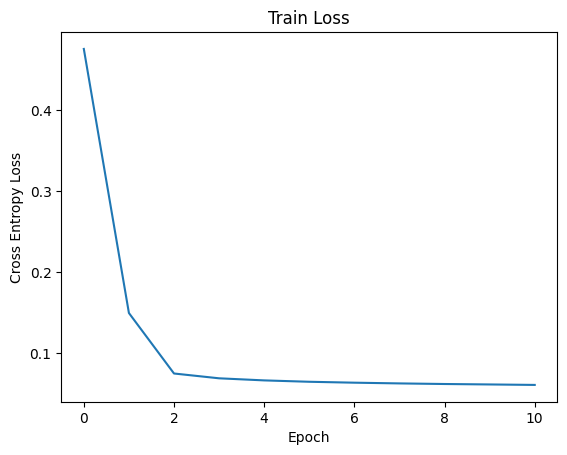
\includegraphics[width=0.6\linewidth]{loss.png}}
\caption{Model training loss}
\label{fig}
\end{figure}


\begin{figure}[htbp]
\centerline{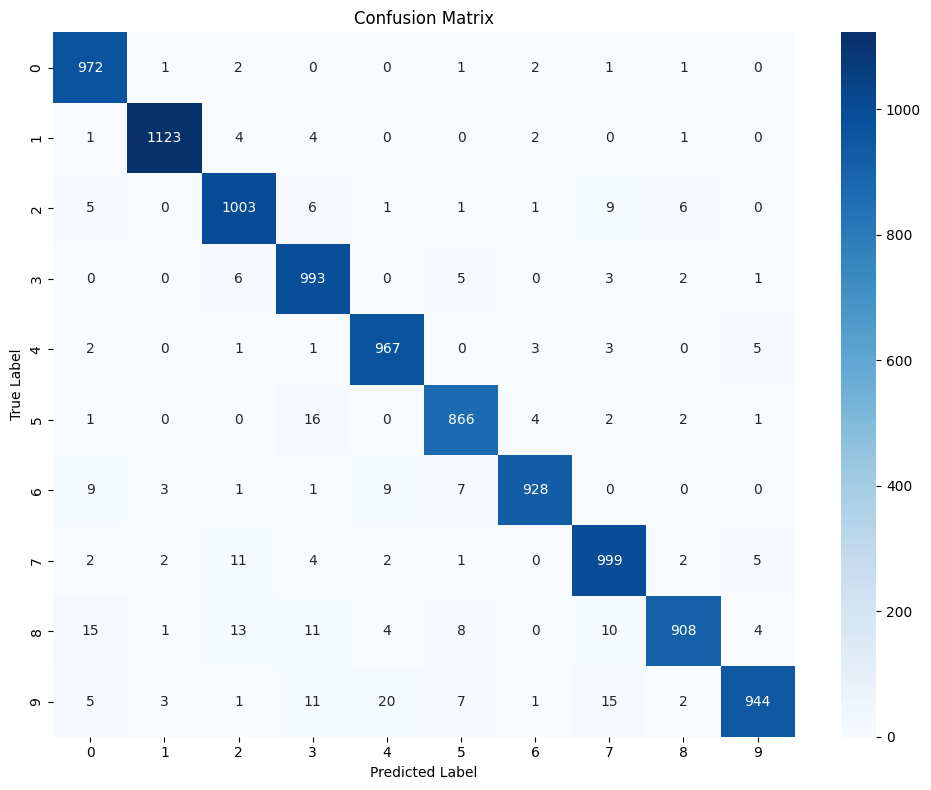
\includegraphics[width=0.85\linewidth]{confusion matrix.png}}
\caption{Confusion matrix on the test set}
\label{fig}
\end{figure}


\begin{table}[htbp]
\caption{Classification metrics on train set}
\begin{center}
\begin{tabular}{|c|c|c|c|c|c|c|}
\hline
& \multicolumn{2}{|c|}{\textbf{Precision}} & \multicolumn{2}{|c|}{\textbf{Recall}} & \multicolumn{2}{|c|}{\textbf{F1}} \\
\hline
& Train & Test & Train & Test& Train & Test \\
\hline
0 & 0.97 & 0.96 & 0.99 & 0.99 & 0.98 & 0.98  \\
1 & 0.99 & 0.98 & 0.99 & 0.99 & 0.99 & 0.99  \\
2 & 0.98 & 0.96 & 0.98 & 0.97 & 0.98 & 0.97  \\
3 & 0.96 & 0.95 & 0.98 & 0.98 & 0.97 & 0.97  \\
4 & 0.97 & 0.96 & 0.98 & 0.98 & 0.98 & 0.97  \\
5 & 0.97 & 0.97 & 0.98 & 0.97 & 0.97 & 0.97  \\
6 & 0.99 & 0.99 & 0.98 & 0.97 & 0.98 & 0.98  \\
7 & 0.97 & 0.96 & 0.98 & 0.97 & 0.98 & 0.97  \\
8 & 0.98 & 0.98 & 0.96 & 0.93 & 0.97 & 0.96  \\
9 & 0.98 & 0.98 & 0.94 & 0.94 & 0.96 & 0.96  \\
\hline
Train Accuracy & \multicolumn{6}{|c|}{0.976}  \\
\hline
Test Accuracy & \multicolumn{6}{|c|}{0.970}  \\
\hline
\end{tabular}
\label{tab1}
\end{center}
\end{table}

In the Table \ref{tab1} we benchmark the execution performance of the same LeNet5 model with PyTorch and our implementation. We use the MNIST dataset with batch size of 600 images to calculate the metrics. We can see that our implementation uses 33\% less memory compared to PyTorch. However, our model implementation does the forward and backward operation noticeably slower than PyTorch. The forward take 10 times as long compared to PyTorch. Furthermore, a severe slowdown can see the backward function. While the forward and backward operation of PyTorch take a similar amount of time (0.05 seconds) to complete, the backward pass in our implementation takes 30 times longer.


\begin{table}[htbp]
\caption{Performance comparison}
\begin{center}
\begin{tabular}{|c|c|c|}
\hline
& \textbf{PyTorch} & \textbf{Our Implementation} \\
\hline
\textbf{Memory Usage} & 1.2 GB & 0.8 GB \\
\textbf{Forward time} & 0.05 s & 0.4 s \\
\textbf{Backward Time} & 0.05 s & 1.5 s \\
\hline
\end{tabular}
\label{tab1}
\end{center}
\end{table}


\section{Challenges and Future Works}
In this paper, we have presented the implementation of our Deep Learning framework in Rust. The library is fully written from scratch and self contained with no third party dependencies.
Due to the limited time frame, we were not able to optimize our library which result in a 30 times slow execution time compared to PyTorch. Profiling the model, we saw that the main factor for the slow down was convolution. In the following revision, we will improve and optimize our library especially for convolution. Furthermore, we plan to support computing on GPU in the future. 


\begin{thebibliography}{00}

\bibitem{pytorch} Paszke, A., Gross, S., Massa, F., Lerer, A., Bradbury, J., Chanan, G., ...  Chintala, S. (2019). PyTorch: An imperative style, high-performance deep learning library. In Advances in Neural Information Processing Systems (Vol. 32, pp. 8024–8035). Curran Associates, Inc.

\bibitem{tf} Abadi, M., Agarwal, A., Barham, P., Brevdo, E., Chen, Z., Citro, C., ...  Zheng, X. (2015). TensorFlow: Large-scale machine learning on heterogeneous systems. Retrieved from https://www.tensorflow.org/

\bibitem{pcg} O’Neill, M. E. (2014). PCG: A family of simple fast space-efficient statistically good algorithms for random number generation (Tech. Rep. No. HMC-CS-2014-0905). Harvey Mudd College. https://www.pcg-random.org/pdf/hmc-cs-2014-0905.pdf


\bibitem{mnist} Deng, L. (2012). "The mnist database of handwritten digit images for machine learning research. IEEE Signal Processing Magazine", 29(6), 141–142.

\bibitem{lenet} Yann LeCun et. al. "Gradient Based Learning Applied to Document Recognition"

\bibitem{he} K. He, X. Zhang, S. Ren and J. Sun, "Delving Deep into Rectifiers: Surpassing Human-Level Performance on ImageNet Classification," 2015 IEEE International Conference on Computer Vision (ICCV), Santiago, Chile, 2015, pp. 1026-1034,



\end{thebibliography}


\end{document}